\chapter{Result}
The focus of my implementation has been to minimize the amount of hardware usage,
while meeting the timing constraints provided from the rest of the circuit. The 
clock frequency used on the FPGA has been 100 MHz. A throughput in the scale of 
Gbits/s is sufficient for the current design.

The implemented scrambler processes 16 bytes of data in 11 clock pulses with a 
clock frequency of roughly 100MHz, which would correspond roughly to a throughput
of 1.16 Gbits/s. I don't know if it can deal with 100MHz just yet, but probably. 
The scrambler needs to process the key before scrambling input data. A 
keyexpansion takes roughly 45 clock pulses, and is only performed when a new key 
is sent, which is very seldom.

Här är väl tanken att jag ska skriva lite om hur jag implementerat
och bearbetat allt relevant som har med implementationen att göra. 
Vad jag gjort som blivit bättre än andra lösningar. Vad jag fokuserat
på (throughput kontra mängd använd hårdvara).

\section{Problems}
Encountered problems:

\begin{itemize}
\item Not possible to get the license for CSA3
\item Small interrest for CSA3
\item Next to no documentation of the CISSA algorithm
\item Hard finding reliable test vectors
\item Merging
\item Timing
\item Latches
\end{itemize}

Most of these problems are, in my mind, self-explanatory. The one that 
I will discuss here is my problem with merging. This problem occured 
due to the fact that I started the project by implementing small 
entities, that were to be used in higher hierarchies, instead of what 
signals would be needed to be sent from different entities to 
eachother, as well as what they would actually mean.

The pro of my method of working has been that I have been able to get 
results quickly. The con is that a large portion of the time has been 
spent on going back to entities that were already functional, and 
reworking them by adding signals, and finding the right timing 
conditions to make sure that they provided nescessary information for 
entities higher up in the hierarchy.

Since I tried to optimize this implementation to just meet the demands 
on speed, while trying to minimize the amount of hardware needed, I 
introduced timing into a circuit that could otherwise be completely 
combinatorial. This has, as expected, introduced quite a bunch of 
timing-issues. I dare say that all of them are gone now, but it is 
quite hard to know without testing the circuit more extensively.

When I first synthesized the circuit, towards the end of the 
implementation, I found that the circuit synthesized a large amount of 
latches. This made my circuit take up roughly 15\% of the FPGA, and use 
11830 Flip-Flops. There were roughly 3000 latches.
When I managed to remove all of them, my entire circuit used roughly 8\%
of the FPGA, and used about 4500 Flip-Flops instead.

This is the entire hardware usage, including the interface towards the 
FPGA, which is one of the reasons why it might appear large, when 
compared to other implementations.

\section{Hardware}
The top entity can be viewed in Figure \ref{b:scr}, and the rest of 
the entities can be viewed in appendix \ref{app:blocks}.

\begin{figure}
  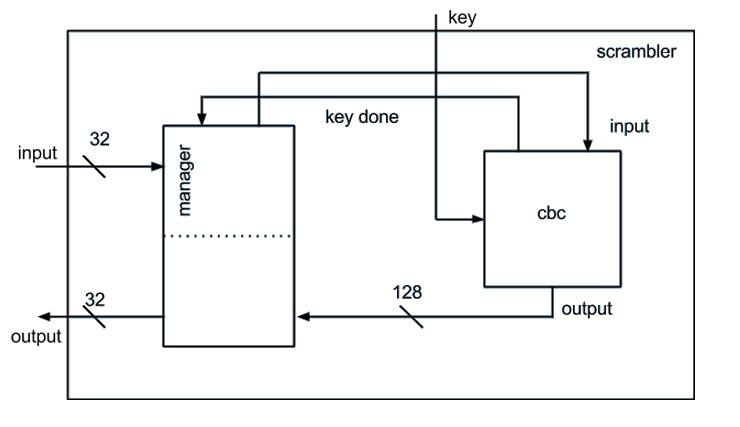
\includegraphics[width=\textwidth]{scrambler}
  \caption{The top entity}
  \label{b:scr}
\end{figure}

\subsection{Hardware usage}
I've run three rounds of synthesis on my circuit. The first two ones 
were performed on the entire scrambler, including the manager 
(interface towrads the rest of the FPGA), while the last synthesis was 
performed on each block of the circuit seperately.

\subsubsection{First synthesis}
The circuit after the first synthesis used up 15\% of the FPGA, and had 
quite a large amount of unnescessary latches and flip-flops included. 

\subsubsection{Second synthesis}
The synthesis report said that 8\% of the FPGA was occupied by the 
circuit. The keyblock3 entity, as well as keyblock1 entity 

\section{Further development}

\subsection{SBox}
The Rijndael Sbox implemented in my design does not synthesize into a 
ROM, which it should be able to do, alternatively into a couple of LUT6.
I have not been able to find out why my code 

\section{Implementation}
My design is very hierarchical. The top layer is an aes128 block in 
CBC-mode. It takes an input TS-packet, selects data from it which it 
scrambles, and then outputs the data in the form of a TS-packet once 
again.

The scrambler consists of two entities. An entity which I call the 
cbc-entity, which deals with the scrambling of the received data. The 
other entity is a data-manager. The manager deals with reading data 
from the interface towards the rest of the FPGA as well as sending the 
right data-bits to the CBC-entity. It also tells the CBC-entity how to 
handle the data, since different things are to be done depending on if 
the data is the first data packet sent, or not.

\subsection{Manager entity}
The manager (Figure \ref{block:manager}) consists of a FIFO, an FSM and 
a couple of registers. The FIFO is needed since the data sent to the 
scrambler from the FPGA is sent in bursts. The FIFO therefore writes 
the data bursts into a memory, from which it later reads, processes and 
sends the data to the CBC-entity. The data written to the FIFO is 
written in packets of 32 bits, but are read 8 bits at the time. The 
manager looks through the data packets to see if there is an adaptation 
field or not, since that changes the way we handle the data. The 
payload is written to the first set of registers as the data is found, 
and then sent to the next set of registers. This is simply done to 
allow the manager to deal with two sets of data in parallell. When the 
packet is ready to be sent, a flag is set and the data is sent to the 
CBC-entity. 

\subsection{CBC entity}
The CBC-entity (Figure \ref{block:cbc}) consists of three small 
entities. An XOR, a multiplexer and a cipher-entity. The multiplexer is 
needed since we want to input the first plaintext into the XOR together 
with an IV. We want to use the output ciphertext instead of the IV for 
the rest of the plaintexts contained within the same TS-packet. There 
is only going to be one aes128 cipher in the CBC-entity, in order to 
save hardware. It will be run in sequence instead of in parallell, even 
though it might reduce the maximal speed of the circuit.

\subsection{Cipher entity}
The aes-128 cipher-entity (Figure \ref{block:cipher}) consists of 4 
components. The data2state entity, which transforms the array into a 
matrix of data. A keyexpansion entity, which takes an input of a key, 
and generates an extended key as an output. An entity, which I chose to 
call rounds, which deals with the encryption of the 16 byte blocks. And 
finally a state2data entity, which transforms the data-matrix into an 
array once again. The cipher entity itself keeps track of timing mainly 
between the keyexpansion and the round entity, and makes sure to 
provide the round entity with the correct roundkey at the right time.

\subsection{Keyexpansion entity}
The keyexpansion-entity is divided into 3 keyblock entities. The first 
keyblock entity decides what 4 bytes of the expanded key we want to 
expand. The second keyblock entity is the keycore, which is only 
performed on every 4th set of 4 bytes. The third keyblock entity 
performs an xor and an incrementation of the internal counter used as 
an index when accessing 4 byte blocks of data.

\subsubsection{Keycore entity}
The keycore entity consists of four entities. Rotword, Sbox, Rcon and a 
counter. The counter is used to get the right data-byte from the Rcon 
entity, and the index is only used in the keycore, and is thus best 
suited to be placed inside the keycore entity. Rotword rotates the 
bytes of the input one step to the left. Sbox replaces the input bytes 
according to the Rijndael Sbox. The Rcon entity both collects the 
correct rcon value from a precalculated vector, as well as inputs it 
into an xor together with the input.

\subsection{Round entity}
The round-entity (Figure \ref{block:round}) consists of four entities. Subbytes, 
shiftrows, mixcolumns and addroundkey. Addroundkey is a somewhat special XOR. 
Subbytes is an Rijndael Sbox, which takes an input 16-byte state, substitutes 
it, and outputs another 16-byte state. Shiftrows transposes the rows of the 
second, third and fourth row of the state. Last, but not least, is the 
mixcolumns entity. It consists of 16 mulblock entities. The input state of 
mixcolumns is split into columns, and each column is sent to a mulblock entity, 
which multiplies the inputs with 1, 2 or 3, then performs a bitwise XOR on them, 
outputting the result of the XOR. The function of the mixcolumns block is a 
rather complex matrix multiplication.

\subsubsection{Addroundkey entity}
Addroundkey is an entity which takes different inputs depending on 
what round we are currently dealing with. On the first round, addroundkey takes 
the input to the round entity. On the last round, it takes the output from the 
subbytes entity. The input to addroundkey is the output from mixcolumns the rest 
of the time.

\subsubsection{The mulblock entity}
The mulblock entity consists of one mul3 entity and one mul2 entity, which 
performs a special kind of hardware multiplication of 3, and 2, on the input. It 
also takes two inputs which it leaves alone. The four results are then XOR:ed 
with eachother, and returned to the mixcolumns entity. The result is then input 
into the correct index in the matrix. 

Mul3 means multiplication with 3, and mul2 means multiplication with 2. A 
multiplication with 2 is a left-shift, followed by an XOR with the fix value 0x1B
if the shifted value exceeds 0xFF. A multiplication with 3 is the same as a 
multiplication with 2, followed by an XOR with the input value.

\section{Tests}
All of the entities in the design have been simulated and evaluated seperately 
before being merged and tested together, to make sure that they had the desired 
functionality both seperately and when combined together. The simulations for the
seperate blocks are trivial, and therefore not included in the report.

Figure \ref{test:1} through \ref{test:3} are tests performed on the complete 
aes-128 block, before CBC-mode. In the figures, in\_key is the input key to be 
extended and used, and datapacket is one packet from a TS. Test vector 1 and 2 
are taken from \citep{AES:2001}, while test vector 3 is generated using a 
webpage.

\emph{Test vector 1 (Figure \ref{test:1})}\\
Input key: 2b 7e 15 16 28 ae d2 a6 ab f7 15 88 09 cf 4f 3c\\
Plaintext: 32 43 f6 a8 88 5a 30 8d 31 31 98 a2 e0 37 07 34\\
Ciphertext: 39 25 84 1d 02 dc 09 fb dc 11 85 97 19 6a 0b 32

\begin{figure}
  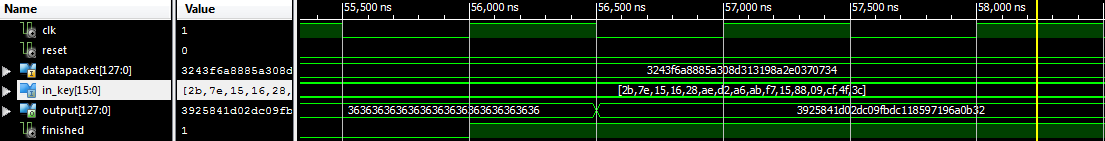
\includegraphics[width=\textwidth]{successtv1}
  \caption{Test vector 1}
  \label{test:1}
\end{figure}

\emph{Test vector 2 (Figure \ref{test:2})}\\
Input key: 00 01 02 03 04 05 06 07 08 09 0a 0b 0c 0d 0e 0f\\
Plaintext: 00 11 22 33 44 55 66 77 88 99 aa bb cc dd ee ff\\
Ciphertext: 69 c4 e0 d8 6a 7b 04 30 d8 cd b7 80 70 b4 c5 5a

\begin{figure}
  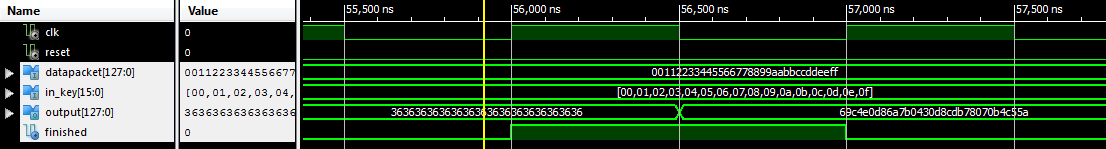
\includegraphics[width=\textwidth]{successtv2}
  \caption{Test vector 2}
  \label{test:2}
\end{figure}

\emph{Test vector 3 (Figure \ref{test:3})} \\
Input key: 10 20 30 40 50 60 70 80 90 a0 b0 c0 d0 e0 f0 bb\\
Plaintext: 00 11 22 33 44 55 66 77 88 99 aa bb cc dd ee ff\\
Ciphertext: bf 99 1f aa 8b 0f e6 48 36 46 a0 2d 33 9e de a5

\begin{figure}
  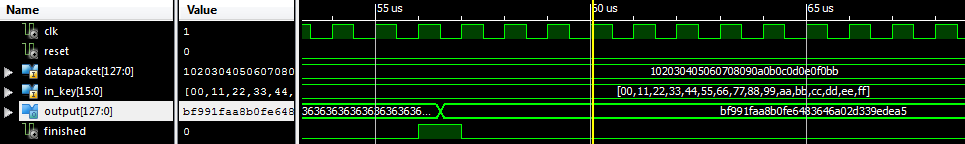
\includegraphics[width=\textwidth]{successtv3}
  \caption{Test vector 3}
  \label{test:3}
\end{figure}
